\documentclass[a4paper,10pt]{article}

\usepackage[spanish]{babel}
\usepackage[utf8]{inputenc}
\usepackage{bookman}
\usepackage{color}
\usepackage{graphicx}
\usepackage[pdftex=true,colorlinks=true,linkcolor=black,urlcolor=blue,plainpages=false]{hyperref} 


%opening
\title{Informe de Proyecto I}
\author{Lorenzo Fundaró - Germán Jaber}


\begin{document}

\begin{figure}[t]
\begin{center}
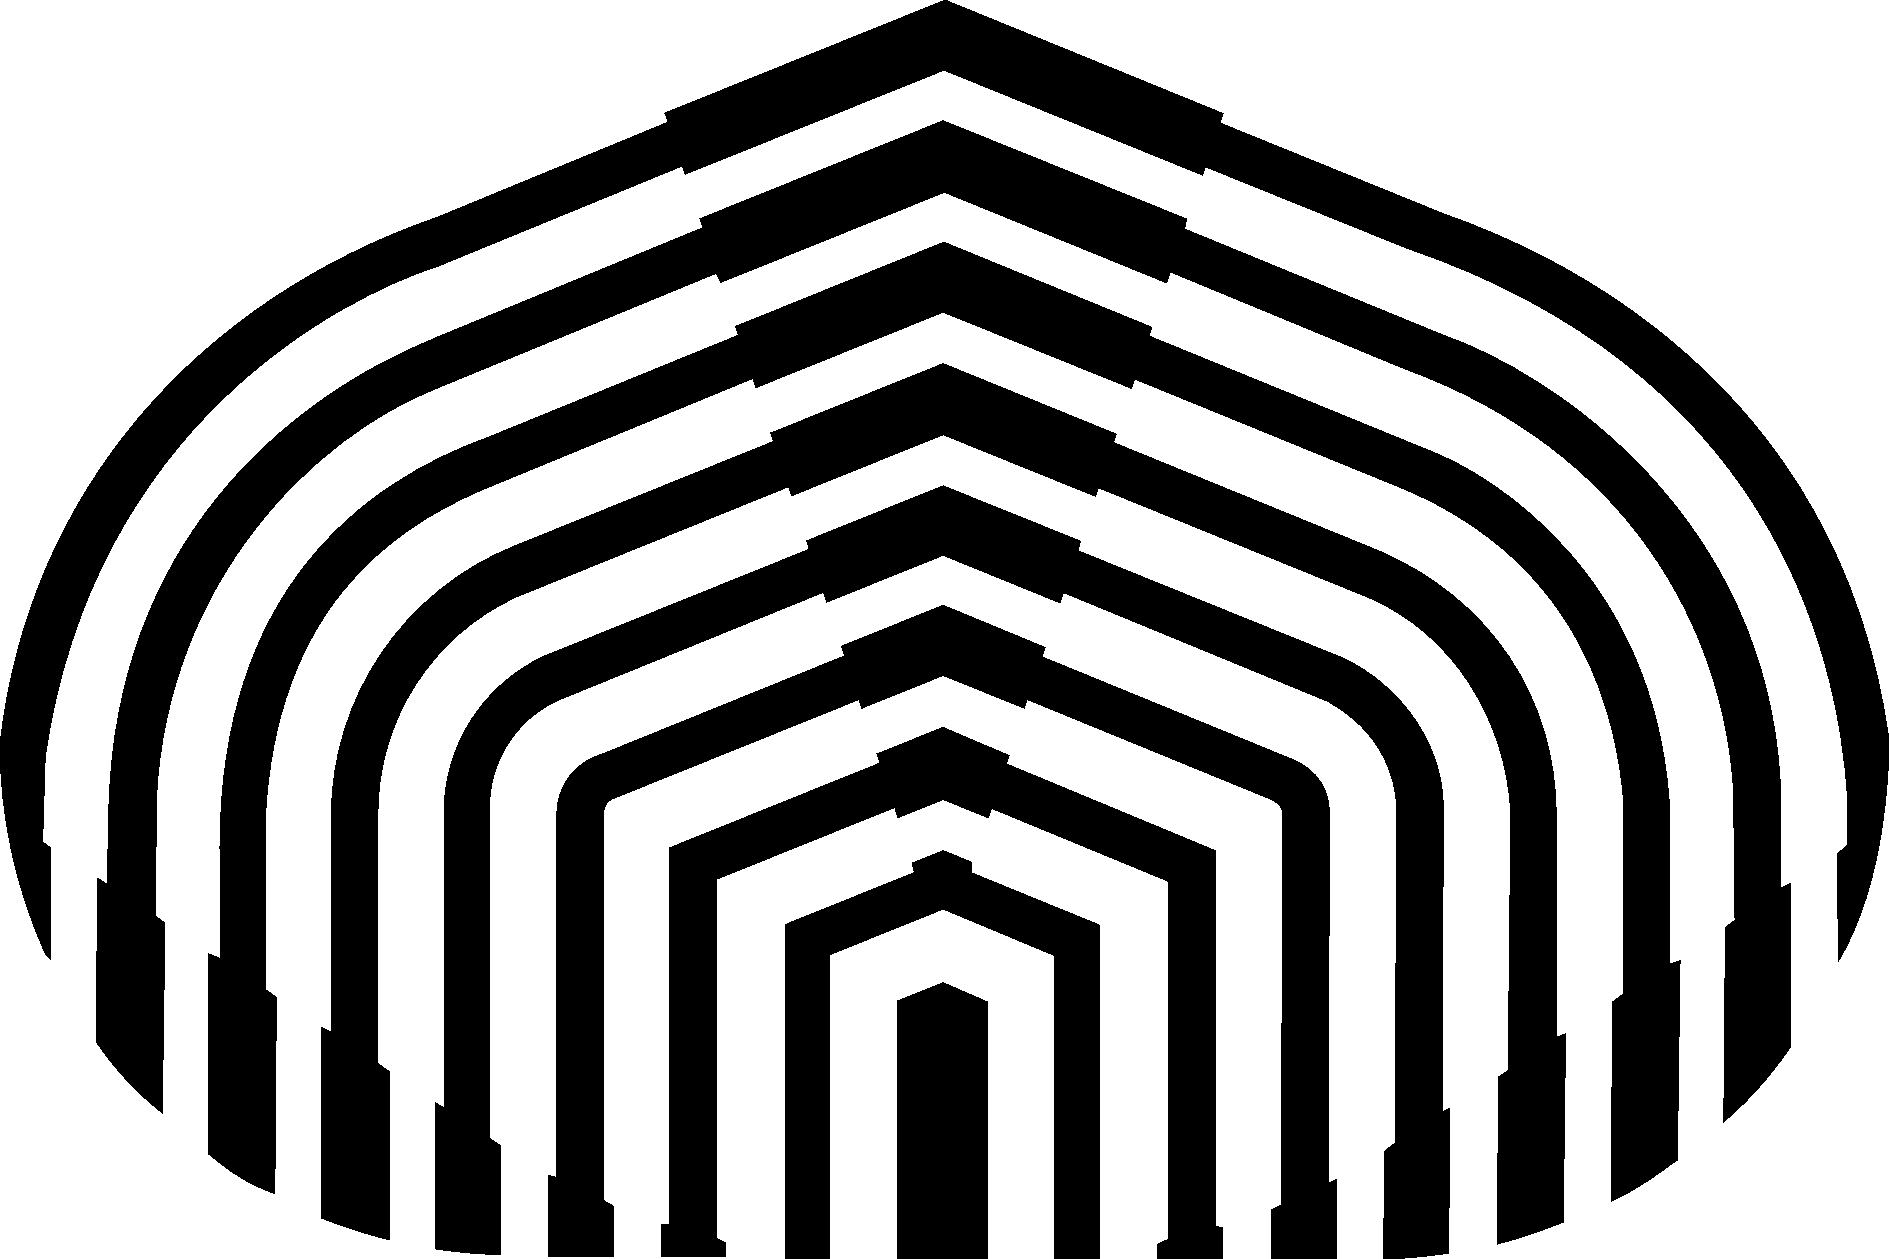
\includegraphics[scale = 0.75]{usb.png}
\end{center}
\begin{center}
\large Universidad Simón Bolívar
\end{center}
\begin{center}
 \large Diseño de Algoritmos I
\end{center}


\end{figure}


\maketitle


\thispagestyle{empty}
\newpage

\tableofcontents{}
\newpage


\section{Introducción}

\subsection{Motivación del Proyecto}
Encontrar la coloración mínima es un problema de comoplejidad NP. 
Sus soluciones son ampliamente aplicadas en casos de la vida real, a nombrar:
\begin{itemize}
 \item Problema de planificación de horarios
 \item Asignación de frecuencia a radios móviles.
 \item Ubicación de registros en la computadora.
 \item Análisis de datos arqueológicos y biológicos
\end{itemize}
Por éstas razones el problema de coloración mínima en un grafo se hace 
interesante hasta el punto de tratar de resolver dicho problema con 
algoritmos optimizados.

\subsection{Breve descripción del problema}
El problema consiste en encontrar la coloración mínima de un grafo. Dicho problema se e aborda con ayuda de la combinación los algoritmos 
Brelaz+Interchange y Enumeración Implícita. El primer algoritmo es 
usado para encontrar las cotas tanto superior como inferior con las que 
el algoritmo de Enumeración Implícita puede encontrar una solución optimal
al problema de coloración mínima. 

\subsection{Descripción del contenido del informe}
En este informe se explica el concepto de diseño que se utilizó
para lograr el objetivo, así también como los detalles de implementación, 
instrucciones de operación, estado actual, conclusiones y referencias bibliográficas.

\section{Diseño}

\subsection{Descripción y justificación del modelo utilizado para representar el problema}
Para representar el grafo en el computador se utilizó una matriz de adyacencias que consta 
de un arreglo de igual tamaño al número de vértices del grafo. Cada casilla de dicho arreglo es 
una estructura que consta del vértice que lo representa, un apuntador a una lista enlazada de adyacencias, 
un color, y un arreglo que llamamos color-around. Se decidió utilizar un arreglo ya que proporciona acceso 
constante a sus elementos. Para las adyacencias no se usó un arreglo ya que cada vez que se requiere saber los 
adyancetes a un vértice dado siempre es necesario recorrer la estructura que se implemente de forma lineal, por lo que 
una lista enlazada se perfilaba como la mejor opción ya que no desperdiciaría espacio, mientras que una matriz nxn 
hubiese gastado espacio que nunca sería utilizado en caso de tener un grafo poco denso. 

\subsection{Estructuras de datos y algoritmos involucrados en la aplicación}

\subsubsection{Estructuras de datos}
\begin{itemize}
 \item \textbf{Linked-List}:  Tipo lista enlazada que contiene un entero que representa un vértice y un apuntador
 a la próxima estructura de lista enlazada. Esta estructura se eligió por su uso eficiente de memoria.
 \item \textbf{Row-vertex}: Estructura que se utiliza para representar
la matriz de adyacencias. El apuntador a linked-list
sirve para apuntar la estructura de nodos adyacentes
al vértice vertex. El apuntador a entero llamado
color-around es una estructura que permite saber
cuáles son los colores que el vértice vertex tiene
en sus adyacencias.
 \item \textbf{Tuple}: Tupla que sirve para representar los vértices con su 
 grado en el arreglo ordenado por grados que pide DSTATUR.
 \item \textbf{Pair}: Pair es la estructura que retorna Dsatur.
Clique representa la cota inferior de coloración.
Coloring representa la cota superior.
Members es un arreglo que contiene los miembros
que conforman la clique máxima encontrada por el algoritmo
 \item \textbf{Linked-Array-list}: contiene un apuntador a arreglo, un color, y un apuntador a otra estructura 
de tipo \textbf{Linked-Array-list}. Es utilizada para guardar componentes en conjuntos vectoriales.
\end{itemize}

\subsubsection{Algoritmos involucrados}

\begin{itemize}
 \item \textbf{Dsatur+interchange}: para el ordenamiento decreciente de los vértices se utilizó el Algoritmo Quicksort. Los 
grados de saturación sólo se actualizan para los vértices que no han sido coloreados, de esta manera se ahorra costo 
de operaciones. El algoritmo recibe un argumento llamado start-point el cuál es -1 para indicar que se quiere hayar 
la cota superior y recibe algún número mayor o igual que cero hasta el número de vértices del grafo cuando se quiere encontrar 
la clique máxima (cota inferior).
Para encontrar la clique máxima el algoritmo cada vez que introduce un nuevo color incrementa la cota inferior. Si se repite algún color de los ya utilizados entonces no modificamos la cota inferior. Sin embargo, a partir de que se introduzca un nuevo color se verifica si el nuevo vértice coloreado hace clique con algunos de los vértices que ya 
sabemos que pertenecen a una clique. Éste método de ampliación de cliques nos permite tener mejores cotas inferiores que 
resultan ser muy útiles para el algoritmo de enumeración implícita cuando se aplica la optimización de no permutar 
los elementos que se sabe pertenecen a la clique máxima encontrada por el algoritmo de Dsatur+Interchange.


\begin{itemize}
 \item \textbf{get-max-degree}: función que en caso de ocurrir una igualdad en los números de saturación devuelve el próximo
vértice no coloreado de grado mayor.
\item \textbf{update-satur}: modifica estructuras de datos en vértices adyacentes a v(sub)i. En el momento que se colorea un vértice v(sub)i todos los adyacentes a éste sufren un aumento 
de saturación siempre que el color utilizado no sea el de uno adyacente a un adyacente de v(sub)i. Si el grado 
de saturación de un elemento es -1 significa que dicho elemento ya fue coloreado. Por otro lado, se aprovecha de 
colocar en 1 la casilla de color-around que corresponde al color utilizado por v(sub)i.
 \item \textbf{leasp-color}: retorna el menor color posible. Dado un vértice v(sub)i que se quiere colorear se utiliza la estructura color-around. Sobre ésta se itera desde el principio hasta conseguir alguna casilla en 0 (indicando la ausencia del color i en la casilla).
\item \textbf{repeated}: algoritmo que en caso de encontrar una repetición de grados de saturación devuelve el próximo vértice de grado mayor no coloreado.
\end{itemize}
\item \textbf{Degree}: prepara los vértices en una estructura vértice-grado llamada tupla, luego todos estos elementos se almacenan en un arreglo de tuplas llamado deg-vert.
\item \textbf{Compare}: función de comparación utilzada por Quicksort.
 \item \textbf{Enumeración-Implícita}: este algoritmo prosigue tal como se enuncia en el proyecto. Sin embargo se le agregó la optimización de fijar los elementos que pertenecen a la clique máxima encontrada por Brelaz+Interchange teniendo que permutar sólo los elementos que no pertenecen a dicha clique reduciendo así el umbral de soluciones.
Otra optimización que se consideró utilizar pero no se llegó implementar consiste en tratar de seguir ampliando 
la clique que tenemos fija. Cómo sabemos que encontrar la clique máxima de un grafo es un problema NP, no podemos 
esperar que Brelaz+Interchange nos dé la clique máxima. Sin embargo mientras consideramos todas las permutaciones sí existe la posibilidad de encontrar la clique máxima. Para ampliar el arreglo de elementos fijos es necesario entonces hacer una verificación similar a la que hicimos en Brelaz+Interchange para ampliar la clique, es decir,en una permutación 
cualquiera, cada vez que se introduce un nuevo color se puede verificar si el vértice coloreado hace clique con los elementos que no permutamos. Ésta optimización permite seguir podando el árbol de permutaciones.
\begin{itemize}
\item \textbf{update-color-around}: función que actualiza el arreglo color-around que indica a un vértice v(sub)i cuáles son 
los colores que tiene a su alrededor.
\item \textbf{get-vertices}: función que retorna un arreglo de vértices en el que se tiene en las primeras j casillas los vértices que conforman la clique máxima encontrada por Brelaz+Interchange. Luego en las N-j casillas restantes se tiene el resto de los elementos que serán permutados por implicit-enum.
\item \textbf{move-vertex}: función auxiliar a get-vertices que permite mover los vértices de una clique máxima al principio del arreglo vértices.
\item \textbf{color-fixed}: función que colorea los elementos fijos del algoritmo de enumeración implícita.
\item \textbf{check-perm}: dado que nuestro algoritmo para encontrar permutaciones es iterativo, es necesario un mecanismo que permita saber si hemos alcanzado la última permutación posible para un arreglo dado. Esta verificación es importante porque de lo contrario la implementación del algoritmo de Dijkstra se hace inestable.
\end{itemize}

\item \textbf{twoOnN}: algoritmo que cálcula la combinatoria de 2 elementos en número de colores utilizados.
\item \textbf{interchange}: se calculan las componentes por medio de un DFS en los nodos. Se verifica la condición de intercambio 
y se hace el intercambio en caso de proceder.
\end{itemize}
\newpage
\section{Detalles de Implementación}

\subsection{Reseña de los elementos implementados, problemas encontrados y solución}

\subsubsection{Representación y Actualización Del Grafo}


Para la representación del grafo el principal desafío fue poder actualizar coloración y saturación rápidamente, incluso después de un intercambio.

El grafo esta representado como un arreglo de listas de adyacencias. Cada índice representa un nodo, los cuales enumeramos a partir de cero. Cada índice del arreglo guarda el color del nodo, un apuntador a su lista de adyacentes y un apuntador a un arreglo que guarda la cantidad de vecinos que tienen un determinado color al que llamaremos \textbf{color-around}, hablaremos de \textbf{color-around} más adelante.

Las listas de adyacentes solo contienen el índice del vecino en el arreglo de listas de adyacencias. Estas listas ameritan ser liberadas de memoria en tiempo O(Grado del grafo).

El color se guarda como un entero, ya que también numeramos los colores desde el cero. Para nodos no pintados, el color es -1.

color-around contiene, para el indice i, el numero de vecinos que están coloreados con el color i. Este arreglo es tan largo como el número de vértices de grafo.

Además de esta estructura, también mantenemos un arreglo, llamado degree-vert, que mantiene un registro de la saturación de los nodos del grafo. degree-vert contiene para el índice i, la cantidad de colores distintos adyacentes al vértice i. Este arreglo también es tan largo como nodos tenga el grafo.

El hecho de que las listas solo guarden el índice del vecino y el hecho de que el color se guarde directamente en el arreglo con las listas de adyacencias nos permite actualizar el color de un nodo en O(1).

color-around combinado con degree-vert nos permite actualizar la saturación en O(grado(i)), siendo grado(i) la función que devuelve el grado del vértice i. Cuando se colorea un nodo, basta con chequear para cada vecino si ya tenían referencias al nuevo color del nodo, si no tenían tales referencias se aumenta en uno(1) su grado de saturación en degree-vert, luego se aumenta en uno(1) el numero de referencias en color-around. Cuando se cambia el color de un nodo basta con (para cada vecino) restar en color-around uno(1) a las referencias del color viejo, y si llegase a cero, se disminuye la saturación en degree-vert en uno(1), la actualización por el color nuevo es igual a cuando se colorea un nodo por primera vez.

\subsubsection{Intercambio}

Hubo dos temas cruciales en el diseño de intercambio, uno fue la búsqueda y representación de las componentes inducidas por los dos colores elegidos, el otro fue el cálculo de todas las combinaciones de dos colores del conjunto de colores adyacentes el nodo del intercambio.

Encontrar componentes en esta estructura puede lograrse, gracias a las listas enlazadas, en O(Nodos alcanzables desde el punto de partida), usando DFS o BFS. Nosotros elegimos DFS por su simplicidad.

Para guardar las componentes encontradas en intercambio se usa una lista enlazada simple que contiene apuntadores a arreglos. Estos arreglos se crean de tamaño igual a la cantidad de vértices del grafo y se utilizan como conjuntos vectoriales (1 si el elemento esta, 0 en caso contrario). Estos arreglos vectoriales nos permiten revisar rápidamente si un nodo pertenece o no a una componente y llenarlos también es fácil y rápido. Su desventaja es que ameritan que sean liberados de memoria cuidadosamente y en tiempo O(Número de componentes).

Nunca vimos la necesidad de inducir un grafo. La exploración en un grafo inducido la pudimos lograr discriminando que nodos examinar viendo sus propiedades.

Para el cálculo de las combinaciones de colores ideamos un algoritmo que solo funciona para calcular combinatorias de dos elementos, pero que solo amerita un(1) intercambio para obtener siguiente combinación. La desventaja de este algoritmo es que requiere de una pequeña estructura de control para que pueda funcionar a través de varias llamadas la función que lo contiene.

El algoritmo se basa en el hecho de que, una vez que se combina un elemento con todos los demás elementos de su conjunto, se puede dejar de considerar ese elemento en las combinaciones posteriores, y se puede operar recursivamente sobre lo que sobra del conjunto.

\subsubsection{Enumeración Implícita}
Un problema importante fue calcular las permutaciones, queríamos un algoritmo iterativo y no recursivo para el resolver el problema, así que usamos el algoritmo de Dijkstra, el cual para una permutación genera la próxima permutación en orden lexicográfico.
En cuanto al flujo del algoritmo de enumeración implícita se le agregó la optimización de sólo permutar los elementos que no pertenecen a la clique máxima encontrada por Brelaz+Interchange.
\newpage
\section{Instrucciones de Operación}

\subsection{Código fuente de aplicación}
El código fuente se puede conseguir en el archivo tar.gz que viene con éste informe.

\subsection{Descripción detallada de como compilar y correr la aplicación}

\subsection{¿Cómo descomprimir el archivo tar.gz?}
En una cónsola de linux se debe ejecutar el siguiente comando:
\begin{verbatim}
 tar -vzxf Grupo6.tar.gz
\end{verbatim}
A continuación se crea una carpeta llamada Grupo6 dónde se encuentran los archivos fuentes del proyecto.

\subsection{¿Cómo compilar?}
En una cónsola de linux debe dirigirse a la carpeta donde estan los archivos fuentes, desde allí se deberá ejecutar
el siguiente comando:
\begin{verbatim}
 make all
\end{verbatim}
Con esto se compilan todas las fuentes. En caso de querer borrar los archivos generados por la compilación se procede hacer:
\begin{verbatim}
 make clean
\end{verbatim}

\subsection{¿Cómo ejecutar?}
En la carpeta de archivos fuentes se provee de un script llamado script.sh. Si se quieren ejecutar todas las instancias 
el comando debe ser el siguiente:
\begin{verbatim}
 ./script.sh resultado
\end{verbatim}
donde resultado es el nombre del archivo donde se escribirán los resultados de la corrida. Si se quiere, éste archivo puede recibir cualquier nombre diferente a resultado.
Si se quiere ejecutar una instancia particular se procede con el siguiente comando:
\begin{verbatim}
 ./main < grafos/instancia-particular
\end{verbatim}
\newpage
\subsection{¿Cómo interpretar resultados?}
Cada instancia arroja un resultado con la siguiente estructura:
\begin{verbatim}
1 Grafo 14-0,9-1.col
2 Resultados de Brelaz+Interchange
3 Cota superior = 9
4 Cota inferior = 7
5 Resultado de enumeración implícita 
6 Número cromático = 9 
7 Tiempo en segundos de ejecución del programa: 96.2635
\end{verbatim}
Explicación de cada línea:
\begin{enumerate}
 \item Nombre de la instancia, el primer número indica el la cantidad de vértices, el segundo la densidad y el tercero el número de archivo.
\item Indicador de algoritmo
\item Coloración arrojada por Brelaz-Interchange
\item Cota inferior. Clique máxima encontrada al aplicar Brelaz-Interchange N veces.
\item Indicador de algoritmo
\item Número cromático encontrado por enumeración implícita.
\item Tiempo en segundos según función provista en el proyecto
\end{enumerate}
Si Brelaz-Interchange arroja una cota superior igual a la inferior entonces el algoritmo de enumeración implícita 
no se ejecuta.

\section{Estado Actual}
\subsection{Indicación del estado final de la aplicación}
El proyecto funciona correctamente para todas las instancias. La optimización de fijar los elementos pertenecientes a la clique máxima de Brelaz+Interchange hace que sólo 6 instancias excedan los 5 minutos. 
\subsection{Errores}
Problemas al liberar memoria en el algoritmo de Enumeración Implícita.
\newpage
\section{Otros}
\subsection{Demostración formal de Enumeración Implícita}
Supongamos que G es un grafo cualquiera y que su número cromático es N.
Supongamos que K(sub)g es una coloración mínima de G que utiliza k colores llamados k1, k2...kn

   Existe una permutación P de los vértices de G tal que todos los vértices de un color ki están contiguos en P.
      Si se tomaran los vértices de G en el orden de P pero sin colorear y se utilizara la estrategia greedy de colorear con el menor color posible. Se obtendría una coloración mínima de G.
      
      Dado que el algoritmo de enumeración implícita prueba todas las permutaciones, eventualmente probará ésta. En el mejor caso, la solución óptima se igualará con la cota inferior y devolverá la coloración mínima, en el peor caso explorará todas las permutaciones y devolverá la cota superior, que es la coloración mínima.
      Debido a que la cota inferior se actualiza en base a cliques en el grafo, podemos estar seguros de que nunca se van a perder soluciones podando el árbol usando la cota mínima.
      Como la cota superior se crea en base a soluciones completas, podemos asegurar que la coloración mínima nunca las excederá, por lo también es seguro podar el árbol en base a la cota superior.


Si existiera una clique o parte de una clique al principio de las permutaciones consideradas que estuviera fija (es decir, que no se permutara), esto tampoco afectaría al algoritmo si esta clique está bien coloreada. Esto debido a que podemos estar seguros de que la coloración de esa porción del grafo es optimal.

\subsection{Ejemplo de Brelaz+Interchange sin solución óptima}
Si se corre el proyecto para la instancia 12-0,5-3.col la coloración que resulta de aplicar Brelaz+Interchange 
es 5. Sin embargo aplicando el algoritmo de enumeración implícita se puede notar que la coloración mínima del grafo
es de 4 colores.
\newpage
\subsection{Tabla de resultados}
\newpage

\section{Conclusiones y recomendaciones}
El algoritmo de Dsatur-Interchange es útil para dar unas cotas de referencia al algoritmo de enumeración implícita. Sin 
embargo el algoritmo de enumeración implícita tarda una cantidad considerable de tiempo si no se aplica ningún tipo de optimizaciones que logren 
reducir el umbral de las soluciones. Se recomienda seguir las recomendaciones planteadas en la sección de Algoritmos involucrados donde se describe en el punto de enumeración implícita unas mejoras para podar el árbol de soluciones.

\section{Referencias Bibliográficas}
\begin{itemize}
 \item http://nicolas-lara.blogspot.com/2009/01/permutations.html (consultada el 17-02-10)
\item http://en.wikipedia.org/wiki/Petersen-graph (consultada el 17-02-10)
\item Meza Oscar, Ortega Maruja. “Grafos y Algoritmos”. Editorial Equinoccio, Universidad Simón Bolívar. 2007. ISBN 980-237232-3
\item Brélaz 1979 Daniel Brélaz. «New Methods to Color the Vetices of a Graph», Communications of the ACM 22-4, 1979, 251-256
\end{itemize}

\end{document}

